% Session 1 -- the charge density wave in real space.
% Placement: sec. "Worked example 1", at the "numerically, this shows up..." paragraph.
% Rendered by figures/blender/s01f04_cdw.py, labels in figures/overlays/s01f04_cdw.tex.
\begin{aqmfigure}{fig:s01:cdw}{The charge density wave of the chain (1.6), solved in mean field for
a periodic chain of eight sites at half filling. The height of the liquid in each cup is the charge
$\langle n_i\rangle$, and next to each chain is its single-particle spectrum, with an electron on
every occupied level and degenerate levels side by side. In front, at $V=0$, every site has the same
charge and the spectrum is gapless, since the Fermi level is inside a pair of degenerate levels.
Behind, the nearest-neighbor repulsion drives the mean-field instability (here $V=3t$), and the
charge accumulates on alternating sites, which doubles the unit cell, drawn as the translucent slab,
and opens a gap in the spectrum. The Hamiltonian is translationally symmetric in both cases, but the
ground state behind is not.}
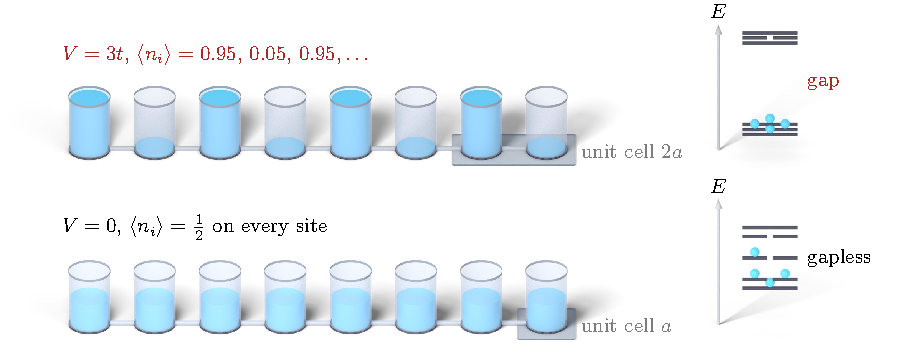
\includegraphics{figures/pdf/s01f04_cdw.pdf}
\end{aqmfigure}
